\chapter{Linearna regresija}

Vinkove rezultate iz kemije so založili. Enostavno, komisija je
izgubila izpitne pole. Rešitev: Vinko bo kemijo pisal še
enkrat. Ampak, ne more, je ravno odšel na trening odbojke v
Rio. Ravnatelj pravi, da je tako ali tako vseeno, ker da eksterci ne
štejejo. Bi pa razredničarka silno želela imeti to oceno, da lahko
Vinka uvrsti v primerno učno skupino. V zbornici je učiteljica fizike
rekla, da so ocene iz kemije tako ali tako podobne tem iz fizike
(slika~\ref{f:fiz-kem-tab}). Zamrmrala je še nekaj okoli regresijskih
modelov in premic, potem pa odšla na mete Galilejeve krogle iz
strehe. Tisti dan je niso več videli.

\begin{table}[htbp]
\caption{Rezultati zunanjega preverjanja za 16 učencev razreda 8.A iz
  fizike in kemije.}
\label{f:fiz-kem-tab}
\begin{center}
\begin{tabular}{lrrrrrrrrr}
\toprule
ime & fiz & kem \\
\midrule
Albert & 46 & 36 \\
Branka & 11 & 22 \\
Cene & 100 & 89 \\
Dea & 90 & 92 \\
Edo & 17 & 12 \\
Franci & 98 & 91 \\
Helena & 81 & 94 \\
Ivan & 33 & 48 \\
Jana & 87 & 91 \\
Leon & 77 & 79 \\
Metka & 78 & 93 \\
Nika & 15 & 5 \\
Polona & 22 & 13 \\
Rajko & 51 & 52 \\
Stane & 92 & 96 \\
Zala & 92 & 67 \\
\bottomrule
\end{tabular}
\end{center}
\end{table}

Vinko je fiziko pisal 70. Razredničarka je lepo prosila za pomoč učiteljico
matematike, ki je bila tisti dan posebej razpoložena. Začnimo z
grafom, pravi. Tistim z ocenami iz fizike in kemije
(slika~\ref{f:fiz-kem}).

\begin{figure}[htbp]
\begin{center}
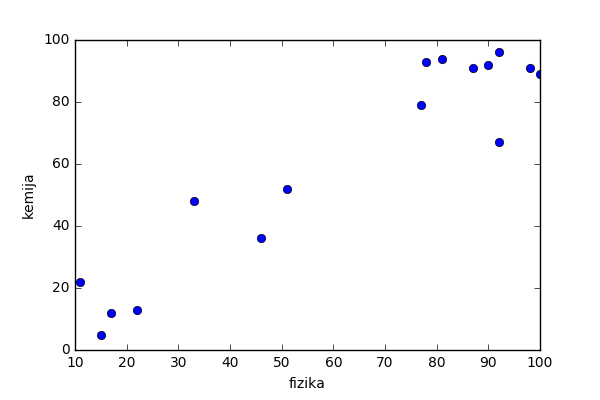
\includegraphics[width=10cm]{slike/fiz-kem.png}
\caption{Ocene fizike in kemije na razsevnem diagramu.}
\label{f:fiz-kem}
\end{center}
\end{figure}

\section{Linearni model ene spremenljivke in kriterijska funkcija}

Učiteljica fizike ima kot kaže prav, ocene kemije in fizike so med
sabo nekako povezane. Tudi učiteljica matematike ima prav: če se le
da skušamo podatke najprej predstaviti v kakšnem grafu. Od tu dalje
bomo poskušali sami. Morda začnemo s premico, ki ji bomo rekli kar
model. Model zato, ker lahko za vsako oceno pri fiziki na podlagi
modela napovemo oceno pri kemiji. Da bo vse skupaj zgledalo bolj učeno
in primerno za univerzitetni študij, označimo oceno pri fiziki s
spremenljivko $x$, oceno pri kemiji, ki jo računamo na podlagi ocene
iz fizike in jo v našem modelu modeliramo pa z $y$. Ocena kemije je
funkcija ocene iz fizike, zato lahko zapišemo:

\begin{equation}
  y = f(x)
\end{equation}

Rekli smo, da bomo zadeve poenostavili in da bo naš model kar
premica. Nekaj takega, kot kaže slika~\ref{f:fiz-kem-priblizno}. Na njej bi iz
ocene fizike 70 ocenili, da bo ocena kemije znašala 62. Ampak, ali je
premica, ki jo kaže slika, res tista ``prava''? Obstaja kakšna boljša
premica, kakšen boljši model? Kako pa sploh ocenimo kvaliteto modela?

\begin{figure}[htbp]
\begin{center}
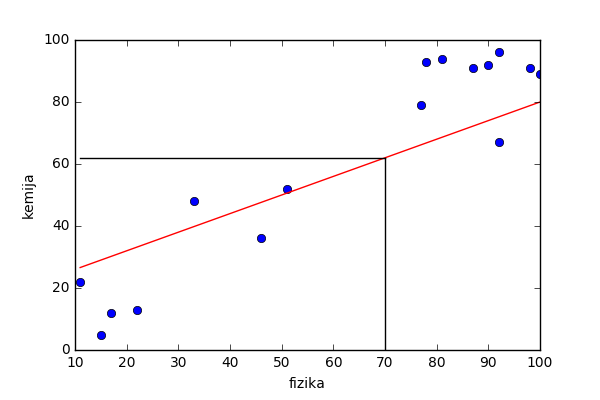
\includegraphics[width=10cm]{slike/fiz-kem-priblizno.png}
\caption{Linearni model, ki iz ocene fizike izračuna oceno za
  kemijo. Za Vinkovo oceno iz fizike 70 predvidi, da je ocena pri
  kemiji enaka 62. Pravilno?}
\label{f:fiz-kem-priblizno}
\end{center}
\end{figure}

Za vsako točko v grafu, vsak znan podatek, torej za vsak par vrednosti
$(x^{(i)},y^{(i)})$ lahko izračunamo napako, ki jo dobimo, ko vrednost odvisne
spremenljivke $y$ napovemo z modelom. Napoved označimo z $\hat{y}$ in
za primer $i$ izračunamo napako napovedi
$\epsilon^{(i)}=\hat{y}^{(i)}-y^{(i)}=f(x^{(i)})-y^{(i)}$. Vse napake za naš dani model in
primere v učni množici smo označili na sliki~\ref{f:fiz-kem-eps}.

\begin{figure}[htbp]
\begin{center}
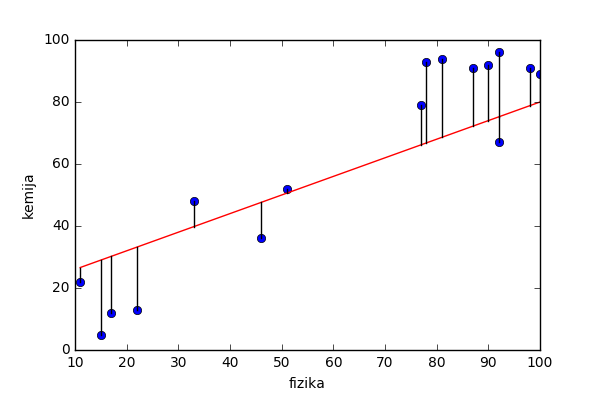
\includegraphics[width=10cm]{slike/fiz-kem-eps.png}
\caption{Napake linearnega modela na učni množici.}
\label{f:fiz-kem-eps}
\end{center}
\end{figure}

Napake $\epsilon^{(i)}$ so lahko pozitivne ali negativne.
Pravzaprav nas predznak ne zanima, zanima nas samo velikost napake. In
če že, nas ne zanimajo tiste majhne napake, ampak nas motijo predvsem
tiste večje, recimo napake pri Zali in Albertu. Radi bi, da bi naš
model bil tak, da bi napake, ki ga naredi pri napovedi primerov iz
učne množice bile čim manjše. Razmišljanje iz tega odstavka lahko
kvantificiramo, oziroma izrazimo numerično s funkcijo:

\begin{equation}
J = {1\over 2m}\sum_{i=1}^m {\epsilon^{(i)}}^2 = {1\over 2m}\sum_{i=1}^m
(\hat{y}^{(i)}-y^{(i)})^2 = {1\over 2m}\sum_{i=1}^m (f(x^{(i)})-y^{(i)})^2
\label{eq:jab}
\end{equation}

Funkcijo $J$ imenujemo {\em kriterijska funkcija}, ker z njo izrazimo
našo preferenco, kakšen model bi radi imeli. Enačba za $J$ je
povprečna kvadrirana napaka. Povprečna zato, da lahko njeno vrednost
primerjamo nad različno velikimi učnimi množicami. Kvadrirana zato,
ker nam je vseeno, ali so napake pozitivne ali negativne in zato, da
izpostavimo večje napake. Tisto dvojko v $1\over 2m$ smo tu dodali kar
tako (ne škodi), kasneje pa se izkaže, da se nam pri kakšni operaciji
okrajša in nam pride prav pri poenostavitvi rezultatov.

Radi bi, da bi bila vrednost kriterijske funkcije $J$ čim
manjša. Najbolje nič. A to vsaj pri naši učni množici z modelom -
premico, ki mu od tu dalj lahko kar rečemo linearni model, ne bo šlo
(če misliš pa, da gre, poskusi).

Premico lahko zapišemo z enačbo:

\begin{equation}
  y=f(x)=a x + b
\end{equation}

S tem, ko poznamo model, naša kriterijska funkcija postane funkcija
dveh parametrov, parametra $a$ in parametra $b$:

\begin{equation}
  J(a, b) = {1\over 2m}\sum_{i=1}^m ((a x^{(i)} + b)-y^{(i)})^2
\end{equation}

Da povzamemo: oceno iz kemije bomo za Vinka ocenili tako, da bomo
zgradili model, ki iz znanih ocen fizike in kemije pridobi
model. Model bo tak, da bo za učno množico, torej za učence, kjer
poznamo ocene iz obeh predmetov, iz ocene fizike izračunal oceno
kemije. Želeli bi tak model, ki je na učni množici čimbolj
natančen. Natančnost ocenimo s kriterijsko funkcijo $J$, katere
vrednost izračunamo iz učnih podatkov in modela. Kriterijska funkcija
je funkcija parametrov modela. Ker gradimo linearni model in ker je
naš model premica v ravnini, sta parametra dva, $a$ in $b$. Želeli bi
torej pridobiti taka parametra, pri katerih je vrednost kriterijske
funkcije najmanjša. Iskanju takih parametrov pravimo optimizacija.

\section{Razmislek o optimizaciji}

Tu se bomo delali, da o optimizaciji še nimamo pojma. (Čeprav to prav
gotovo ni res, saj smo pri matematiki in nekaterih ostalih predmetih
veliko slišali o njej. A nič hudega, da zadevo ponovimo). Recimo da
imamo funkcijo $J(a)$, torej funkcijo parametra $a$, in želimo poiskati
vrednost parametra $a^*$, kjer je vrednost funkcije najmanjša. Dodatno
recimo, da vemo, da je funkcija konveksna. Za konveksne funkcije
velja, da so zvezne in da za vsak interval njene domene (vrednosti
parametra $a$, za naš primer) velja, da vrednost funkcije v srednji
točki intervala ne presega aritmetičnega povprečja vrednosti funkcije
v skrajnih točkah intervala. Po domače, konveksna funkcija enega
parametra ima obliko črke U. Recimo tudi, da funkcije $J(a)$ nimamo
zapisane analitično, a da lahko izvemo oziroma povprašamo po njeni
vrednost za dano vrednost parametra.

Naše iskanje minimuma funkcije $J(a)$ lahko začnemo v neki
točki. Recimo, v točki nič. V tej točki nas pravzaprav raje kot njena
vrednost zanima njen odvod. Če je odvod enak nič (ali pa zelo blizu
ničle), potem vemo, da smo našli pravo vrednost parametra $a$. Če je
odvod pozitiven, vemo da smo s parametrom $a$ desno od optimalne
vrednosti $a^*$, in da je $a^*<a$. Če je odvod funkcije $J(a)$
negativen, bo vrednost $a*$ morala biti večja od trenutne vrednosti
$a$. Odvoda funkcije $J$, torej $dJ(a)/da$ nimamo zapisanega v
analitični obliki. Odvod pri izbrani vrednosti parametra $a$ ni nič
drugega kot naklon funkcije v tej točki, to pa lahko približno
izračunamo tako, da pogledamo, kakšne so vrednosti te funkcije malce
stran od točke $a$, na levo in na desno:

\begin{equation}
  {\Delta J(a)\over \Delta a}\Bigr|_{a} = {J(a+\delta) - J(a-\delta) \over
    2\delta}
\end{equation}

Ko vemo za odvod $J(a)$, lahko našo trenutno rešitev, torej začetno
točko $a$, premaknemo v nasprotni smeri odvoda. Še enkrat, v nasprotni
zato, ker iščemo minimum. Torej

\begin{equation}
  a \leftarrow a - \alpha {dJ(a)\over da}\Bigr|_{a}
\end{equation}

Vrednost $\alpha$ nam določa, za koliko se premaknemo. Tipično lahko
izberemo neko majhno vrednost, recimo $\alpha=0.1$.

Pythonovska implementacija iskanja optimalne vrednosti bi lahko torej
bila nekako takšna:

\begin{python}
def derivative(f, a, delta=1e-3):
    return (f(a+delta) - f(a-delta)) / (2*delta)

a = 8
for _ in range(10):
    a = a - 0.2 * derivative(J, a)
    print("%.2f" % a)
\end{python}

Tokrat smo se odločili, da naše iskanje optimalne vrednosti $a^*$
pričnemo pri $a=8$ in da je $\alpha=0.2$. Za funkcijo

\begin{python}
def J(a):
    return (a-5)**2+3
\end{python}

Dobimo naslednji izpis:

\begin{python}
6.80
6.08
5.65
5.39
5.23
5.14
5.08
5.05
5.03
5.02
\end{python}

Kar je kar fino, saj smo že v desetih korakih prišli precej blizu
prave vrednosti $a^*$. Pravi vrednosti bi se lahko, zaradi
konveksnosti naše kriterijske funkcije, s primernim številom
iteracij in s primerno vrednostjo $\alpha$ poljubno približali.

Pri zgornji optimizaciji smo predpostavili, da odvoda funkcije ne
poznamo. Če bi imeli na voljo funkcijo, ki bi nam neposredno
izračunala odvod, torej tako, da bi ga izračunala brez klica osnovne
funkcije, bi nam bilo še enostavneje in odvoda potem ne bi rabili
ocenjevati. Za dano funkcijo $J(a)$ v zgornjem primeru bi tako lahko
izračunali njen analitični odvod, ter tega uporabili v zapisu funkcije
{\tt derivative}. Bi znal ustrezno spremeniti kodo? Dobiš podobne
rezultate, kot jih dobimo s približkom za odvod?

\section{Iskanje parametrov univariatne linearne regresije}

Tako učeno pravimo modelu - premici, s katerim bomo napovedovali ocene
kemije iz ocen fizike. Univariatne zato, ker je to linearna regresija
nad enim samim atributom $x$ (atribute imenujemo tudi
variate). Linearna zato, ker je povezava med atributi in vrednostjo
modela linearna ($a x + b$). Regresija zato, ker je izhod modela
zvezna vrednost (drugačni od regresijskih modelov bodo
klasifikacijski, ki še pridejo na vrsto).

Pri linearni regresiji iščemo take parametre regresije, torej
parametre modela, ki nam dajo minimalno vrednost kriterijske funkcije
$J$. V prejšnjem razdelku smo si pogledali trik, kako tako vrednost
poiščemo v primeru, ko je $J$ funkcija enega samega parametra. A pri
univariatni analizi je ta funkcija odvisna od dveh parametrov, torej
$J=J(a,b)$. Zato bomo iskanje optimalne vrednosti parametrov $a^*$ in
$b^*$ pričeli pri neki vrednosti teh parametrov, potem pa te vrednosti
popravljali, pač glede na odvod po vsakem od parametrov. Lahko torej
zapišemo:

\begin{eqnarray}
a & \leftarrow & a - \alpha {dJ(a,b)\over da}\Bigr|_{a,b} \\
b & \leftarrow & b - \alpha {dJ(a,b)\over db}\Bigr|_{a,b}
\end{eqnarray}

Pravzaprav kakšne večje spremembe glede na stvari iz prejšnjega
razdelka ni, dela pa je le malce več, ker moramo izračunati odvod po
enem in drugem parametru. Odvod bi lahko izračunali tudi numerično,
tako, kot smo to počeli zgoraj, a ker kriterijsko funkcijo poznamo, ne
bo odveč, da odvod izračunamo analitično. Upoštevamo, da je odvod
vsote enak vsoti odvodov. Spomnimo, odvajamo torej kriterijsko
funkcijo iz enačbe~\ref{eq:jab}, njena odvoda po parametrih $a$ in $b$ sta:

\begin{eqnarray}
  {\partial J(a,b)\over\partial a} &=& {1\over m}\sum_{i=1}^m((a x^{(i)} + b)-y^{(i)})x^{(i)} \\
  {\partial J(a,b)\over\partial b} &=& {1\over m}\sum_{i=1}^m((a x^{(i)} + b)-y^{(i)})
\end{eqnarray}

Pri odvajanju smo izgubili konstanto $2$ v imenovalcu
normalizacijskega člena $1\over 2m$. Omenimo samo, da bi lahko odvoda
zložili v vektor in s tem dobili nekaj, čemur pravimo gradient. Ne se
ustrašit, gradient je čisto preprosta zadeva: funkcijo z več parametri
smo vsakič odvajali po posameznem parametru, in s tem dobili vektor,
ki ga imenujemo gradient funkcije.

Rezultat zgleda zanimivo enostaven, a je bila, navkljub seštevanju,
taka tudi naša kriterijska funkcija. Izpišimo sedaj korak osveževanja
vrednosti parametrov $a$ in $b$, ki jih uporabljamo pri iskanju našega
linearnega modela:

\begin{eqnarray}
a & \leftarrow & a - {\alpha\over m}\sum_{i=1}^m((a x^{(i)} + b)-y^{(i)})x^{(i)} \\
b & \leftarrow & b - {\alpha\over m}\sum_{i=1}^m((a x^{(i)} + b)-y^{(i)})
\end{eqnarray}

Pythonovska koda za ta osvežitveni korak je preprosta in predvideva,
da so podatki shranjeni v seznamih (vektorjih) {\tt x} in {\tt y}:

\begin{python}
def update(a, b, alpha=0.0001):
    cons = alpha / len(x)
    a = a - cons * sum(((a*xi+b)-yi)*xi for xi, yi in zip(x, y))
    b = b - cons * sum(((a*xi+b)-yi) for xi, yi in zip(x, y))
    return a, b
\end{python}

Če našo optimizacijo pričnemo v točki $(0,0)$ je konvergenca relativno
hitra in se do rešitve prebijemo že po nekaj iteracijah:

\begin{python}
a, b = 0, 0
for _ in range(10):
    a, b = update(a, b)
    print("%.3f %.3f" % (a, b))
\end{python}

Zgornja koda namreč izpiše:
\begin{python}
0.479 0.003
0.726 0.005
0.852 0.006
0.918 0.006
0.951 0.006
0.968 0.006
0.977 0.007
0.982 0.007
0.984 0.007
0.985 0.007
\end{python}

Optimalni vrednosti parametrov $a$ in $b$ sta torej (približno)
$a=0.985$ in $b=0.007$, naš model s podatki iz učne množice
pa je prikazan na sliki~\ref{f:fiz-kem-opt-model}.

\begin{figure}[htbp]
\begin{center}
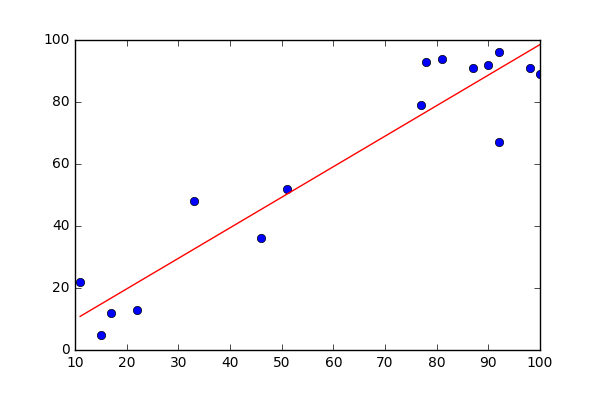
\includegraphics[width=10cm]{slike/fiz-kem-opt-model.png}
\caption{Ocene fizike in kemije na razsevnem diagramu.}
\label{f:fiz-kem-opt-model}
\end{center}
\end{figure}

\section{Multivariatna linearna regresija}

Približek ocene za kemijo izračunan iz ocene za fiziko je sicer čisto
v redu, a našo razredničarko in matematičarko mučijo ostale
ocene. Namreč, zgubila se je ocena za kemijo, vse ostale ocene pa
imamo. Ne samo za fiziko, ampak za slovenščino, matematiko, in
ostale. Bi lahko zgradili linearni model, ki bi upošteval tudi ostale
ocene? Torej, upošteval prav vse ostale atribute, ki so nam na
razpolago. In zgradil linearni model.

Ker imamo sedaj več atributov (variat) gre za multivariatno linearno
regresijo. Najprej nekaj sicer nam že dobro poznane notacije. Naj bo $x$ vektor atributnih vrednosti. Privzemimo, da so vsi atributi zvezni in da imamo $n$ različnih atributov, to je $x_1, x_2,\ldots x_n$. Označimo odvisno spremenljivko z $y$. Naš cilj je na podlagi učnih primerov, to je parov atributnih vektorjev in vrednosti odvisne spremenljivke $(x,y)$ zgraditi model:
%
\begin{equation}
h_\theta(x)=\theta_0 + \theta_1 x_1 + \ldots + \theta_n x_n
\end{equation}
%
Tokrat smo namesto parametrov $a$ in $b$ parametre modela označili s
črko $\theta$, ter parametrom modela dodali tudi indeks. Parameter
$\theta_0$ ustreza prejšnjemu parametru $b$, $\theta_1$ pa parametru
$a$. Da bo zapis bolj enostaven, določimo tudi $x_0$ ki naj vedno, to je, za vse primere, zavzame vrednost 1. Potem lahko zapišemo:
\begin{equation}
h_\theta(x) =\sum_{i=0}^n \theta_i x_i
\end{equation}
oziroma v vektorski obliki
\begin{equation}
h(x)=\theta^T x
\end{equation}

Parametre modela $\theta$ želimo izbrati tako, da bo napaka naše napovedi čim manjša. Napaka napovedi za $i$-ti primer, kjer je $\hat{y}^{(i)}$ napovedana vrednost, $y^{(i)}$ pa prava vrednost odvisne spremenljivke, je
%
\begin{equation}
\epsilon^{(i)}=\hat{y}^{(i)}-y^{(i)}=h_\theta(x^{(i)})-y^{(i)}
\end{equation}
%
Model smo tokrat označili s simbolom $h$, ker model predstavlja
hipotezo nad našimi podatki. Napake v negativno in pozitivno smer
obravnavamo enako, zato je kot prej tudi tu najbolje, da napako kar
kvadriramo. Zanimajo nas taki parametri, pri katerih je kvadrat napake
na učni množici minimalen, oziroma kjer se model čimbolj prilega učnim
podatkom:
\begin{equation}
\min_\theta\sum_{i=0}^m(h_\theta(x^{(i)})-y^{(i)})^2
\end{equation}

Na podlagi zgornjega kriterija zapišimo kriterijsko funkcijo. Kriterij
pomnožimo z $1\over 2$, da nam bo lažje kasneje pri izpeljavi odvodov, ter z $1/m$ da vrednost kriterijske funkcija ne bo odvisna od števila primerov:
%
\begin{equation}
J(\theta)={1\over 2m}\sum_{i=0}^m(h_\theta(x^{(i)})-y^{(i)})^2
\end{equation}
%
Naš cilj je sedaj poiskati take vrednosti parameterov, pri katerih bo
kriterijska funkcija $J(\theta)$ minimalna, oziroma take vrednosti,
pri katerem se bo glede na našo izbrano kriterijsko funkcijo naš
model čim bolje prilegal dani učni množici. 

\section{Metoda najhitrejšega spusta}

Iskanje optimalnih parametrov začnimo v neki točki, na primer kar v
$\theta=\vec{0}$. Potem spreminjamo $\theta$ tako, da se $J(\theta)$
zmanšuje, to je, v nasprotni smeri parcialnega odvoda kriterijske
funkcije. Enako, kot smo počeli v prejšnjem poglavju z parametroma $a$
in $b$, le da tokrat ta korak zapišemo splošno za parameter $\theta_i$:
\begin{equation}
  \theta_i\leftarrow\theta_i-\alpha{\partial\over\partial\theta_i}J(\theta)
\end{equation}
%
Konstanto $\alpha$ imenujemo stopnja učenja, njena vrednost pa bo
narekovala, kako hitro bomo hiteli proti cilju. Če bo vrednost
$\alpha$ prevelika, je možno, da bomo preleteli cilj in se odstrelili v
neskončnost. Če bo vrednost premajhna, bo konvergenca počasna.

Izpeljimo sedaj vrednost parcialnih odvodov oziroma vrednost
gradienta, ko parcialne odvode zložimo v vektor. Pri tem zaenkrat privzemimo, da bomo vrednosti parametra $\theta_i$ prilagodili enemu samemu primeru $(x,y)$:
%
\begin{eqnarray}
{\partial\over\partial\theta_i} J(\theta) & = & {\partial\over\partial\theta_i} {1\over 2m}(h_\theta(x)-y)^2 \\
& = & 2{1\over 2m}(h_\theta(x)-y){\partial\over\partial\theta_i}(h_\theta(x)-y) \\
& = & {1\over m}(h_\theta(x)-y){\partial\over\partial\theta_i}(\theta_0 x_0 + \ldots + \theta_i x_i + \ldots \theta_n x_n - y) \\
& = & {1\over m}(h_\theta(x)-y)x_i
\end{eqnarray}
%
Vsakokratni popravek parametra $\theta_i$ bo tako:
\begin{equation}
  \theta_i\leftarrow\theta_i-{\alpha\over m}(h_\theta(x)-y)x_i
\end{equation}
oziroma za vse primere:
\begin{equation}
  \theta_i\leftarrow\theta_i-{\alpha\over m}\sum_{j=1}^m(h_\theta(x^{(j)})-y^{(j)})x_i^{(j)}
\end{equation}

Pri linearni regresiji oziroma zgoraj opisanemu pristopu najmanjših kvadratov je $J(\theta)$ kvadratna funkcija z enim samim minimumom, zato se nam o tem, da bi se optimizacija zaustavila v nekem lokalnem minimumu ni potrebno bati. Lahko pa, kot smo že zapisali zgoraj, pri velikih vrednostih $\alpha$ minimum zgrešimo in se pričnemo vse bolj oddaljevati od njega. Pomaga seveda zmanjšanje $\alpha$ na vrednost, pri kateri je optimizacija stabilne in skonvergira k pravi vrednosti parametrov $\theta$.
